
\documentclass{beamer}
\usepackage[latin1]{inputenc}
%\usetheme{Montpellier}
%\usetheme{Boadilla}
%\usecolortheme[RGB={204,51,255}]{structure}
%\usecolortheme[named=purple]{structure}
\usecolortheme[RGB={62,128,62}]{structure}
%\definecolor{reddish}{rgb}{0.3,0.15,0.3}
%\definecolor{light}{rgb}{0.8,0.6,0.8}
%\definecolor{reddish}{rgb}{.5,0.15,0.15}
\definecolor{reddish}{rgb}{0.5,0.3,0.4}
%\definecolor{light}{rgb}{0.8,0.6,0.8}
\definecolor{reddish}{rgb}{.7,0.25,0.25}
\definecolor{greenish}{rgb}{.25,0.8,0.25}
\definecolor{blueish}{rgb}{.25,0.25,0.7}
\definecolor{purple}{rgb}{.5,0.0,0.5}
\usepackage{graphicx}
\usepackage{pstricks}

\newcommand{\btVFill}{\vskip0pt plus 1filll}

\setbeamertemplate{navigation symbols}{}

\newcommand{\crish}{\color{reddish}}
\newcommand{\cgish}{\color{greenish}}
\newcommand{\cbla}{\color{black}}
\newcommand{\cred}{\color{red}}
\newcommand{\cblu}{\color{blue}}
\newcommand{\cgrish}{\color{green}}

\newcommand{\sm}{\color{reddish}$}
\newcommand{\fm}{$\color{black}{}}

\newcommand{\letter}[1]{\color{blue}\texttt{#1}\color{black}}
\newcommand{\binary}[1]{\color{red}\texttt{#1}\color{black}}

\usepackage{tikz}
\usetikzlibrary{arrows,decorations.markings,positioning}
\usepackage{epstopdf}
\usetikzlibrary{fit}
\usepackage{pgfplots}

\title[Information Theory lecture 8]{The mutual information: information theory lecture 9}
\author{COMSM0075 Information Processing and Brain}
\institute{\texttt{comsm0075.github.io}}
\date{October 2020}

\begin{document}

\maketitle

\pgfmathdeclarefunction{gauss}{2}{%
  \pgfmathparse{1/(#2*sqrt(2*pi))*exp(-((x-#1)^2)/(2*#2^2))}%
}


\pgfmathdeclarefunction{uniform}{1}{%
  \pgfmathparse{#1}%
}


\begin{frame}{A probability density is a density}

  The probability density isn't any old function. It is a \cblu{}density\cbla.

\end{frame}

\begin{frame}{Density}
  \begin{center}
    
\includegraphics[width=6cm]{unstretched_armstrong.jpg}
  \end{center}
\end{frame}


\begin{frame}{Density}
  \begin{center}
    
\includegraphics[width=10cm]{stretch-armstrong.jpg}
  \end{center}
\end{frame}


\begin{frame}{Density}
  \begin{center}
    
\includegraphics{unstretched_arm.jpg}
  \end{center}

  \begin{center}
    \begin{tikzpicture}
    \node[](left){$\ldots$};
    \node[right =  1cm of left](zero){};
    \node[above = 1cm of zero](overzero){};
    \node[right = 2.0cm of overzero](overa){};
    \node[below = 1cm of overa](a){};
    \node[right = 1cm of a](right){$\ldots$};
    \draw[thick,draw=blue] (left) -- (zero.center) -- (overzero.center) -- (overa.center) -- (a.center) -- (right);
    \draw[dotted] (zero.center) -- (a.center);
    \end{tikzpicture}
\end{center}  
\end{frame}


\begin{frame}{Density}
  \begin{center}
    
\includegraphics{stretched_arm.jpg}
  \end{center}
  
  \begin{center}
    \begin{tikzpicture}
    \node[](left){$\ldots$};
    \node[right =  1cm of left](zero){};
    \node[above = 0.5cm of zero](overzero){};
    \node[right = 4.0cm of overzero](overa){};
    \node[below = 0.5cm of overa](a){};
    \node[right = 1cm of a](right){$\ldots$};
    \draw[thick,draw=red] (left) -- (zero.center) -- (overzero.center) -- (overa.center) -- (a.center) -- (right);
    \draw[dotted] (zero.center) -- (a.center);
    \end{tikzpicture}
\end{center}
  \end{frame}


\begin{frame}{Density}
  
  \begin{center}
    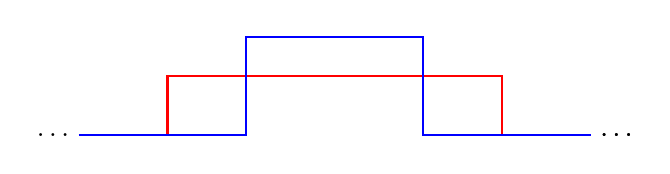
\begin{tikzpicture}
    \node[](left){$\ldots$};
    \node[right =  1cm of left](zero){};
    \node[above = 0.5cm of zero](overzero){};
    \node[right = 4.0cm of overzero](overa){};
    \node[below = 0.5cm of overa](a){};
    \node[right = 1cm of a](right){$\ldots$};
    
    \node[right =  2cm of left](zero2){};
    \node[above =  1cm of zero2](overzero2){};
    \node[right = 2.0cm of overzero2](overa2){};
    \node[below = 1cm of overa2](a2){};
    \node[right = 2cm of a2](right2){$\ldots$};
    \draw[thick,draw=red] (left) -- (zero.center) -- (overzero.center) -- (overa.center) -- (a.center) -- (right);
    \draw[thick,draw=blue] (left) -- (zero2.center) -- (overzero2.center) -- (overa2.center) -- (a2.center) -- (right);
    \end{tikzpicture}
\end{center}
\end{frame}

\begin{frame}{Change of variable}
  \crish
  $$
  P(x\in[x_0,x_1))=\int_{x_0}^{x_1}p_X(x)dx
    $$
    \cbla
Now what happens if we do a change of variable to \crish$y(x)$\cbla.
\end{frame}




\begin{frame}{Change of variable}
  \crish
  $$
  P(x\in[x_0,x_1))=\int_{x_0}^{x_1}p_X(x)dx
    $$
    \cbla
Now what happens if we do a change of variable to \crish$y(x)$\cbla. For simplicity, assume \crish$y(x)$\cbla{} is strictly monotonic so we can invert to get \crish$x(y)$\cbla.
\end{frame}


\begin{frame}{Change of variable}
  Remember how to change variables in an integral:
\crish $$
  dx=\left|\frac{dx}{dy}\right|dy
$$
  \cbla 
so if \crish$y_0=y(x_0)$\cbla{} and \crish$y_1=y(x_1)$\cbla{} we have
\crish
$$
  P(y\in[y_0,y_1))=\int_{y_0}^{y_1} p_X(x(y))\left|\frac{dx}{dy}\right|dy
    $$
\cbla
  
\end{frame}


\begin{frame}{Change of variable - Jacobian}
  Remember how to change variables in an integral:
\cblu $$
  dx=\left|\frac{dx}{dy}\right|dy
$$
  \cbla 
so if \crish$y_0=y(x_0)$\cbla{} and \crish$y_1=y(x_1)$\cbla{} we have
\crish
$$
  P(y\in[y_0,y_1))=\int_{y_0}^{y_1} p_X(x(y))\cblu\left|\frac{dx}{dy}\right|dy
    $$
\cbla
  
\end{frame}


\begin{frame}{Change of variable}
  Remember how to change variables in an integral:
\crish $$
  dx=\left|\frac{dx}{dy}\right|dy
$$
  \cbla
  so if \crish$y_0=y(x_0)$\cbla{} and \crish$y_1=y(x_1)$\cbla{} we have
\crish
$$
  P(y\in[y_0,y_1))=\int_{y_0}^{y_1} \cblu{} p_X(x(y))\crish{}\left|\frac{dx}{dy}\right|dy
    $$
\cbla
\end{frame}


\begin{frame}{Change of variable}

\crish
$$
  P(y\in[y_0,y_1))=\int_{y_0}^{y_1} \cblu{} p_X(x(y))\crish{}\left|\frac{dx}{dy}\right|dy
    $$
\cbla


\begin{tikzpicture}
\begin{axis}[
  no markers, domain=0:10, samples=100,
  axis lines*=left, xlabel=$x$, ylabel=$p_X(x)$,
  every axis y label/.style={at=(current axis.above origin),anchor=south},
  every axis x label/.style={at=(current axis.right of origin),anchor=west},
  height=5cm, width=12cm,
%  xtick={4,6.5}, ytick=\empty,
  xtick=\empty,
  ytick=\empty,
  enlargelimits=false, clip=false, axis on top,
  grid = major
  ]
%  \addplot [fill=cyan!20, draw=none, domain=0:5.96] {gauss(6.5,1)} \closedcycle;
  \addplot [very thick,cyan!50!black] {gauss(4,1)};
%  \addplot [very thick,cyan!50!black] {gauss(6.5,1)};
%\draw [yshift=-0.6cm, latex-latex](axis cs:4,0) -- node [fill=white] {$1.96\sigma$} (axis cs:5.96,0);
\end{axis}

\draw (0,-0.5) -- (10.5,-0.5);
\draw (10.75,-0.5) node{$y$};
  \draw (4,-0.75) node(y){$y$};
  \draw (5,-0.25) node(x){$x$};
  \draw (5,0) -- (5,2.42);
  \draw (6.0,2.65) node(px){\cblu$p_X(x(y))$\cbla};
  \draw (y) -- (x);
\end{tikzpicture}

\end{frame}

\begin{frame}{The $y$ probability density}
  \crish
  $$P(y\in[y_0,y_1))=\int_{y_0}^{y_1} p_Y(y)dy$$
    \cbla
\end{frame}

\begin{frame}{The probability shouldn't change}
\crish
      $$P(y\in[y_0,y_1))=P(x\in[x_0,x_1))$$
    \cbla
\end{frame}



\begin{frame}{The probability shouldn't change}
\crish
      $$P(y\in[y_0,y_1))=P(x\in[x_0,x_1))$$
    \cbla
    so
    \crish $$
\int_{y_0}^{y_1} p_Y(y)dy=\int_{y_0}^{y_1} p_X(x(y))\left|\frac{dx}{dy}\right|dy
$$
\cbla
\end{frame}


\begin{frame}{The probability shouldn't change}

    \crish $$
\int_{y_0}^{y_1} p_Y(y)dy=\int_{y_0}^{y_1} p_X(x(y))\left|\frac{dx}{dy}\right|dy
$$
\cbla
hence
\crish $$
p_Y(y)=\frac{p_X(x(y))}{|dy/dx|}
$$
\cbla
\cblu This behaviour is the definition of a density.\cbla
\end{frame}


\begin{frame}{The entropy is not invariant under a change of variable!}
  \crish
  $$
  h(Y)=h(X)+\int p_X(x) \log_2\left|\frac{dy}{dx}\right|dx
  $$
  \cbla
\end{frame}

\begin{frame}{Scaling}
Using \crish$y=\cblu{}a\crish{} x$\cbla{} in this formula
  \crish
  $$  
  h(aX)=h(X)+\log{|\cblu{}a\crish|}
  $$
  \cbla
\end{frame}

\begin{frame}{The mutual information}
\crish
  $$
  I(X,Y)=h(X)+h(Y)-h(X,Y)
  $$
  \cbla
or
  \crish
  $$
  I(X,Y)=\int p_{X,Y}(x,y)\log_2{\frac{p_{X,Y}(x,y)}{p_X(x)p_Y(y)}}dxdy
  $$
  \cbla
\cbla
\end{frame}



\begin{frame}{The mutual information has nice properties}
\crish
  $$
  I(X,Y)=h(\cblu{}X\crish)+h(Y)\cblu-\crish{}h(\cblu{}X\crish{},Y)
  $$
  \cbla
is invariant under a change of variable; roughly speaking the Jacobian factors cancel!
\end{frame}

\begin{frame}{The mutual information is the same for mutual information}
  \crish
  $$
  I(X^{\delta_x},Y^{\delta_y})\rightarrow I(X,Y)
  $$
  \cbla
as \crish$\delta_x$\cbla{} and \crish$\delta_y$\cbla{} approach zero.
\end{frame}


\begin{frame}{The mutual information is non-negative}
  \crish
  $$
  I(X,Y)\ge 0
  $$
  \cbla
\end{frame}



\begin{frame}{Channel capacity theory}
  \begin{center}
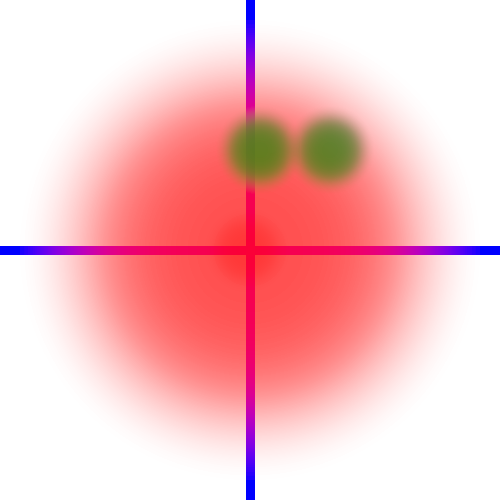
\includegraphics[width=7cm]{cont4.png}
  \end{center}  
\end{frame}


\end{document}

